% ==================== 2 Origin 晶体学计算模板的建立 ====================
\section{Origin 晶体学计算模板的建立}

\subsection{工作簿、列结构与角度单位}

打开 Origin，新建一个工作簿，将其重命名为 \texttt{SIcalculator}，并新增 20 列，使工作表增加到 A--V 共 22 列，如图 \ref{fig:calc-setup}(a)(b) 所示。列数应与模板的列布局一致；后续如需增加计算项目，可在工作表中继续插入行或列。随后按“晶格参数—晶胞体积—倒易参数—晶面指数—结果”的顺序命名各列，如图 \ref{fig:calc-setup}(c) 和图 \ref{fig:calc-formula}(a) 所示。建议的列布局为：

\begin{itemize}[leftmargin=2em,itemsep=1pt]
  \item A--F：$a,b,c,\alpha,\beta,\gamma$；
  \item G：晶胞体积 $V$；
  \item H--M：$a^*,b^*,c^*,\alpha^*,\beta^*,\gamma^*$；
  \item N--S：$h_1,k_1,l_1,h_2,k_2,l_2$；
  \item T--V：$r_1,r_2,\theta$。
\end{itemize}

\begin{figure}[H]
  \centering
  \begin{subfigure}[t]{0.40\linewidth}
    \centering
    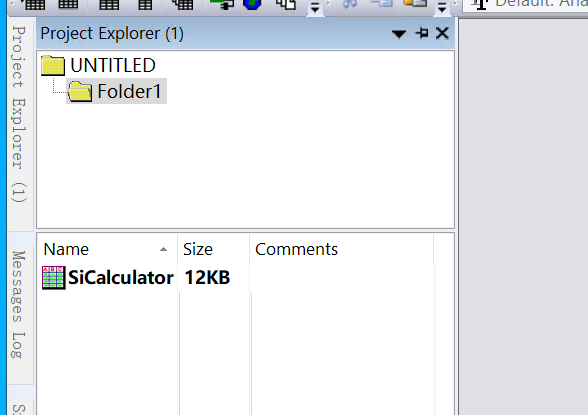
\includegraphics[width=\linewidth]{calc/c01.png}
    \caption{新建工作簿并命名为 \texttt{SIcalculator}}
    \label{fig:calc-setup-a}
  \end{subfigure}\hfill
  \begin{subfigure}[t]{0.30\linewidth}
    \centering
    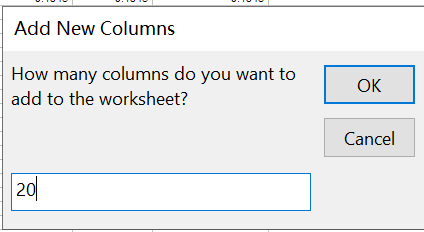
\includegraphics[width=\linewidth]{calc/c02.png}
    \caption{新增 20 列，增加到 A--V 共 22 列}
    \label{fig:calc-setup-b}
  \end{subfigure}

  \vspace{0.4em}
  \begin{subfigure}[t]{0.96\linewidth}
    \centering
    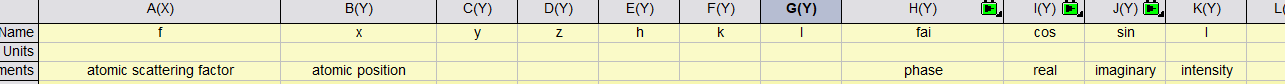
\includegraphics[width=\linewidth]{calc/c03.png}
    \caption{新建列并逐列命名}
    \label{fig:calc-setup-c}
  \end{subfigure}
  \caption{Origin 计算模板的初始设置：(a) 新建并重命名工作簿；(b) 新增 20 列，工作表增加到 A--V 共 22 列；(c) 建立列名。列名将直接作为公式中的变量名使用，因此命名应简洁且不重复。}
  \label{fig:calc-setup}
\end{figure}

需要特别强调角度单位。Origin 的三角函数默认可能使用弧度，而晶体学公式和日常输入都习惯使用角度制。应在 \texttt{Tools $\rightarrow$ Options}（或工作表属性）中把 Angular Unit 设为 Degree，如图 \ref{fig:calc-angle-volume}(a) 所示；否则式 \eqref{eq:volume} 和式 \eqref{eq:angle} 中的 \texttt{cos}、\texttt{acos} 会得到完全错误的结果。这一设置是本模板最容易出错、也最值得先检查的地方。

\begin{figure}[H]
  \centering
  \begin{subfigure}[t]{0.96\linewidth}
    \centering
    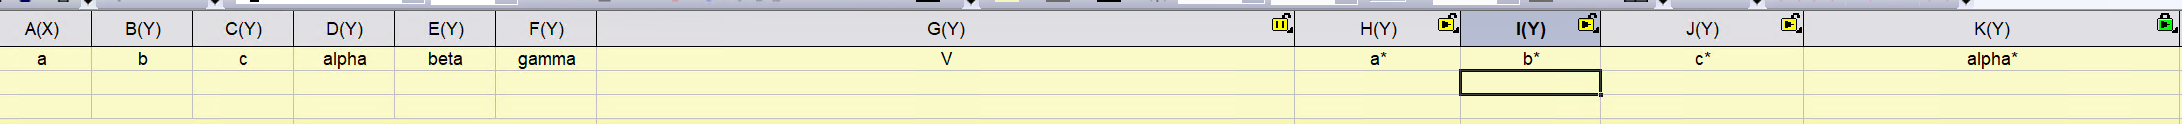
\includegraphics[width=\linewidth]{calc/c04.png}
    \caption{逐行检查并修正列名}
    \label{fig:calc-formula-a}
  \end{subfigure}

  \vspace{0.4em}
  \begin{subfigure}[t]{0.66\linewidth}
    \centering
    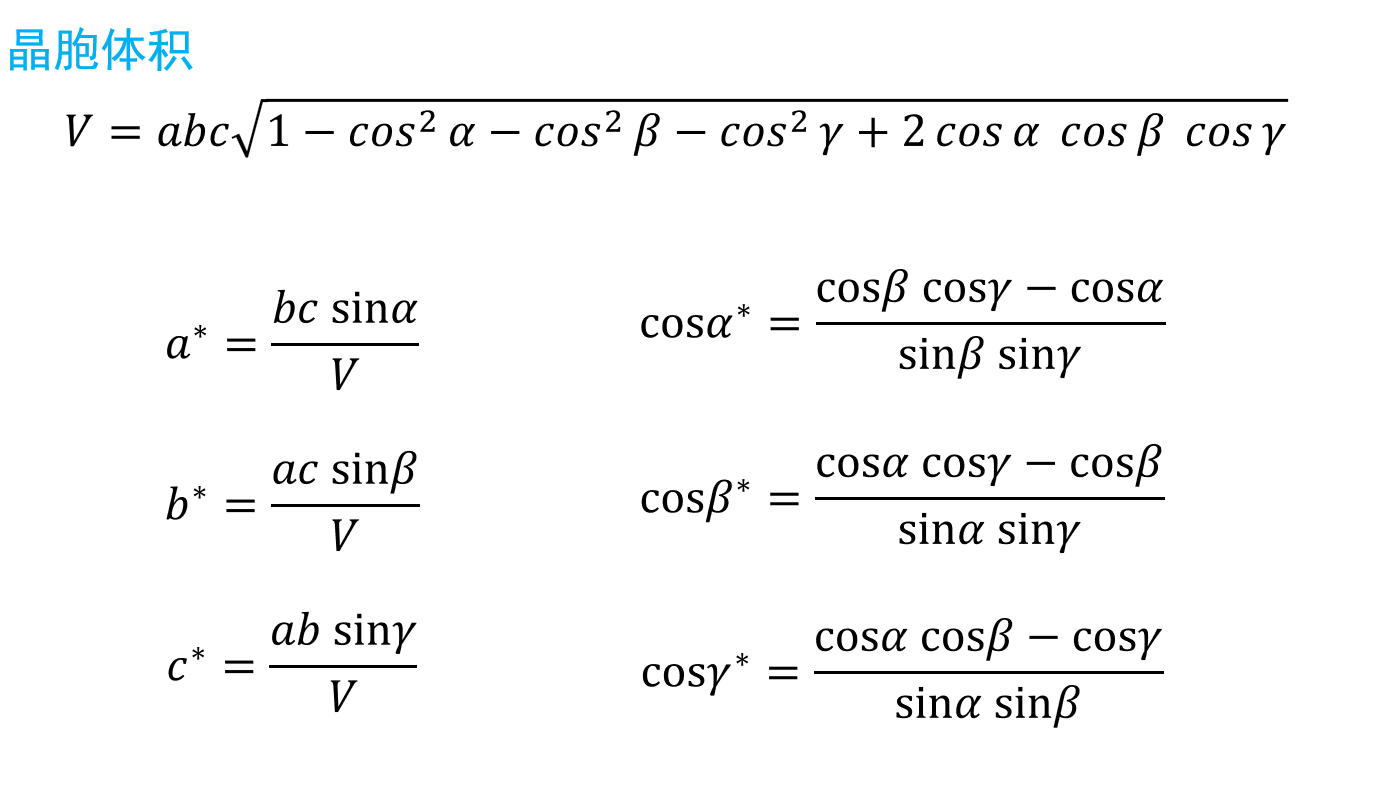
\includegraphics[width=\linewidth]{calc/c05.png}
    \caption{按公式表在对应列输入表达式}
    \label{fig:calc-formula-b}
  \end{subfigure}
  \caption{列名与公式输入。Origin 的公式可直接引用列名（如 \texttt{A}、\texttt{B}），也可引用列序号；使用列名更直观，但改名后公式中的引用必须同步修改。}
  \label{fig:calc-formula}
\end{figure}

\subsection{晶胞体积与倒易点阵参数}

在 A--F 列输入单晶硅的晶格参数：$a=b=c=5.43$，$\alpha=\beta=\gamma=90$，如图 \ref{fig:calc-angle-volume}(b) 所示。选中 G 列，按 \texttt{Ctrl+Q} 打开公式编辑框，输入式 \eqref{eq:volume} 对应的 Origin 表达式
\begin{lstlisting}
A*B*C*sqrt(1-cos(D)^2-cos(E)^2-cos(F)^2+2*cos(D)*cos(E)*cos(F))
\end{lstlisting}
按题目给定的 $a=5.43$~\AA，立方晶系中根号项严格等于 1，因此 $V=a^3=160.103$~\AA$^3$。图 \ref{fig:calc-volume-reciprocal}(a) 的界面数值为 159.22009~\AA$^3$，对应 $a=5.42$~\AA 的旧输入；它恰好说明模板会随 A--C 列的输入而变化，正式计算前应先把晶格参数核对到题目给定值。若体积与 $a^3$ 出现明显偏差，应首先检查角度单位是否误设为弧度。

倒易参数 H--M 列分别输入
\begin{lstlisting}
B*C*sin(D)/G
A*C*sin(E)/G
A*B*sin(F)/G
acos((cos(E)*cos(F)-cos(D))/(sin(E)*sin(F)))
acos((cos(D)*cos(F)-cos(E))/(sin(D)*sin(F)))
acos((cos(E)*cos(D)-cos(F))/(sin(E)*sin(D)))
\end{lstlisting}
其中 H、I、J 三列为 $a^*,b^*,c^*$，K、L、M 三列为 $\alpha^*,\beta^*,\gamma^*$。对单晶硅，模板给出 $a^*=b^*=c^*=0.18416$~\AA$^{-1}$，$\alpha^*=\beta^*=\gamma^*=90^\circ$，如图 \ref{fig:calc-volume-reciprocal}(b) 所示。这与式 \eqref{eq:cubic-reciprocal} 的解析结果一致，可作为模板正确性的第一个自检。

\begin{figure}[H]
  \centering
  \begin{subfigure}[t]{0.32\linewidth}
    \centering
    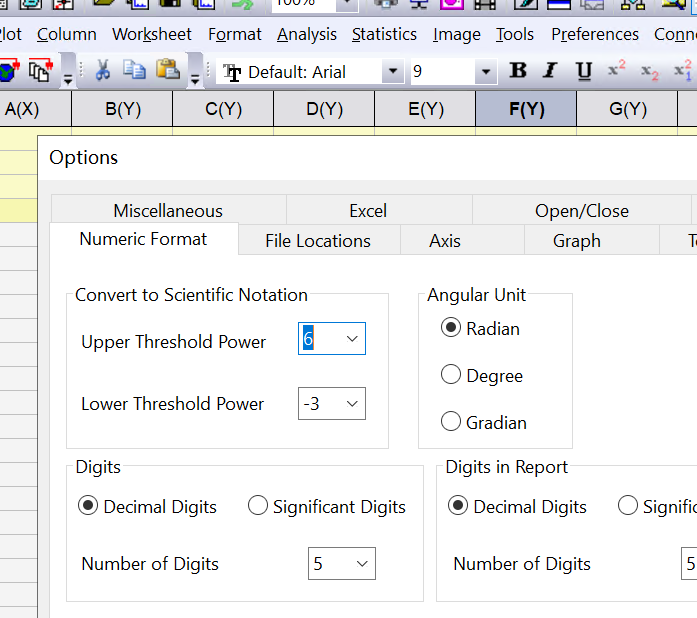
\includegraphics[width=\linewidth]{calc/c06.png}
    \caption{把角度单位设为度}
    \label{fig:calc-angle-volume-a}
  \end{subfigure}\hfill
  \begin{subfigure}[t]{0.12\linewidth}
    \centering
    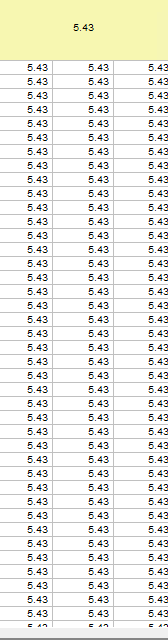
\includegraphics[height=5.4cm]{calc/c07.png}
    \caption{输入 $a,b,c$}
    \label{fig:calc-angle-volume-b}
  \end{subfigure}\hfill
  \begin{subfigure}[t]{0.50\linewidth}
    \centering
    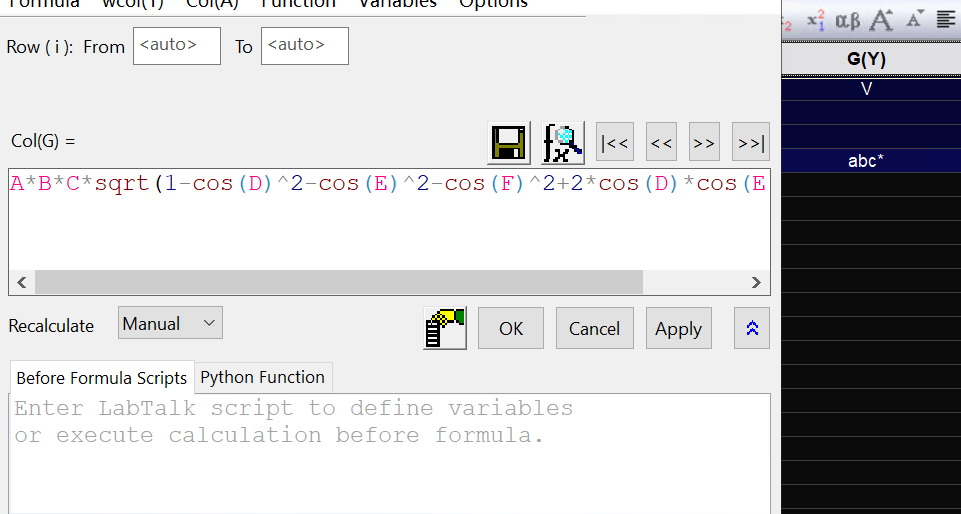
\includegraphics[width=\linewidth]{calc/c08.png}
    \caption{输入体积公式}
    \label{fig:calc-angle-volume-c}
  \end{subfigure}
  \caption{角度单位、晶格参数与体积公式：(a) 将角度单位设为 Degree；(b) 在 A--C 列输入 5.43；(c) 在 G 列输入体积公式。}
  \label{fig:calc-angle-volume}
\end{figure}

\begin{figure}[H]
  \centering
  \begin{subfigure}[t]{0.42\linewidth}
    \centering
    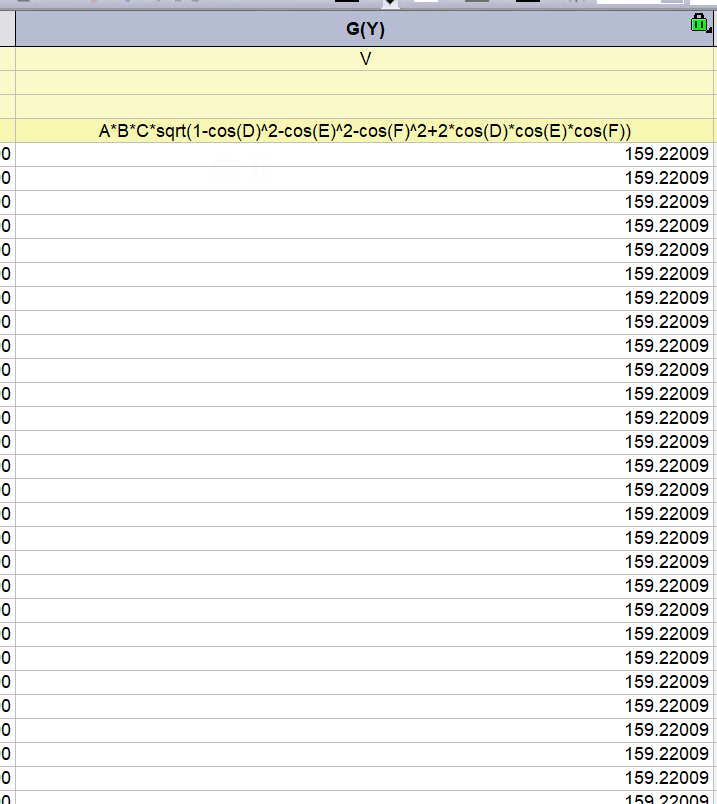
\includegraphics[width=\linewidth]{calc/c09.png}
    \caption{体积计算结果（界面示例；该截图的 159.22009~\AA$^3$ 对应 $a=5.42$~\AA，按题目 $a=5.43$~\AA 计算为 160.103~\AA$^3$）}
    \label{fig:calc-volume-reciprocal-a}
  \end{subfigure}\hfill
  \begin{subfigure}[t]{0.52\linewidth}
    \centering
    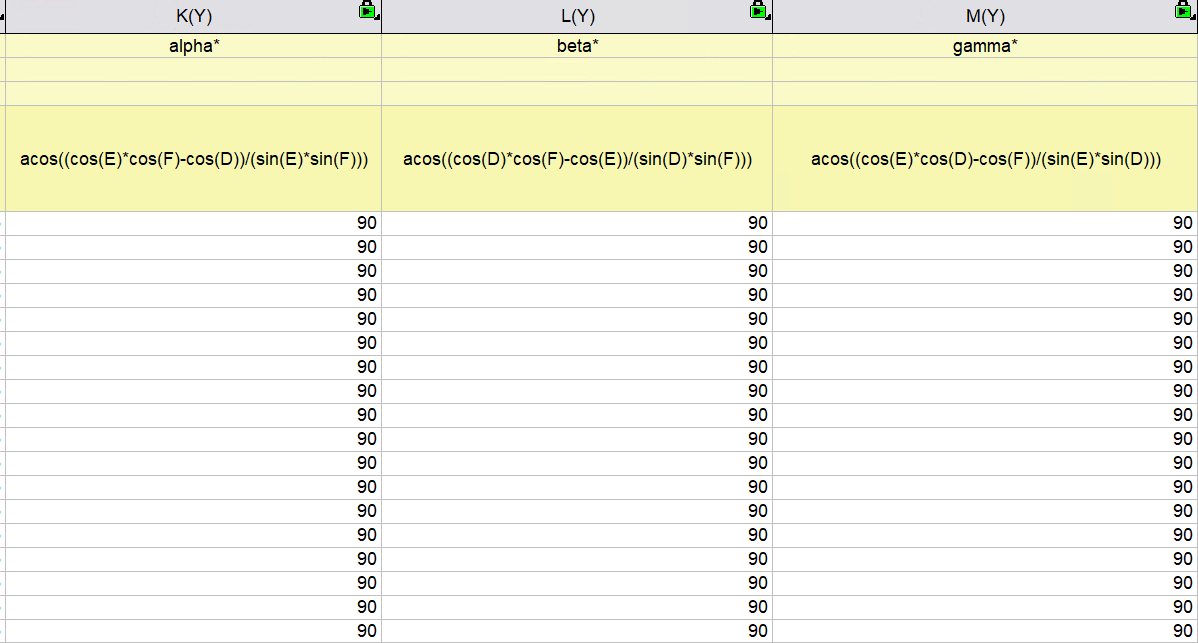
\includegraphics[width=\linewidth]{calc/c10.png}
    \caption{倒易点阵参数与倒易夹角}
    \label{fig:calc-volume-reciprocal-b}
  \end{subfigure}
  \caption{体积与倒易参数的计算结果。立方晶系中 $a^*=b^*=c^*=1/a=0.18416$~\AA$^{-1}$，$\alpha^*=\beta^*=\gamma^*=90^\circ$。}
  \label{fig:calc-volume-reciprocal}
\end{figure}

\subsection{晶面间距、倒易矢量长度与晶面夹角}

在 N--S 列输入两组晶面指数 $h_1k_1l_1$ 和 $h_2k_2l_2$，然后在 T、U、V 三列分别输入
\begin{lstlisting}
SQRT((N*H)^2+(O*I)^2+(P*J)^2+2*N*O*H*I*cos(M)+2*N*P*H*J*cos(L)+2*O*P*I*J*cos(K))
SQRT((Q*H)^2+(R*I)^2+(S*J)^2+2*Q*R*H*I*cos(M)+2*Q*S*H*J*cos(L)+2*R*S*I*J*cos(K))
ACOS((N*Q*H^2+O*R*I^2+P*S*J^2+(N*R+O*Q)*H*I*cos(M)+(N*S+P*Q)*H*J*cos(L)+(O*S+P*R)*I*J*cos(K))/(T*U))
\end{lstlisting}
其中 T、U 分别为 $r_1=1/d_1$、$r_2=1/d_2$，V 为两倒易矢量（即两晶面法向）之间的夹角 $\theta$。图 \ref{fig:calc-rtheta}(a)(b) 给出了输入界面与计算结果；改变 N--S 列的指数，T--V 列会自动更新，因此同一个模板可以反复用于不同的晶面组合。

以 $(h_1k_1l_1)=(423)$、$(h_2k_2l_2)=(232)$ 为例，在 N--S 列输入 4、2、3、2、3、2，T--V 列立即给出对应的 $r_1$、$r_2$ 和 $\theta$。这两个晶面只是任意选取的一组示例，并不对应本作业要求的五个带轴；若要计算某一带轴的基矢，应先按式 \eqref{eq:zone-law} 选取满足 $hu+kv+lw=0$ 的两条反射，具体做法见第 4 章。对立方晶系，也可以直接用解析式校验模板：
\begin{equation}
r_{hkl}=\frac{\sqrt{h^2+k^2+l^2}}{a},\qquad
\cos\theta=\frac{h_1h_2+k_1k_2+l_1l_2}{\sqrt{h_1^2+k_1^2+l_1^2}\sqrt{h_2^2+k_2^2+l_2^2}}.
\label{eq:cubic-check}
\end{equation}

\begin{figure}[H]
  \centering
  \begin{subfigure}[t]{0.22\linewidth}
    \centering
    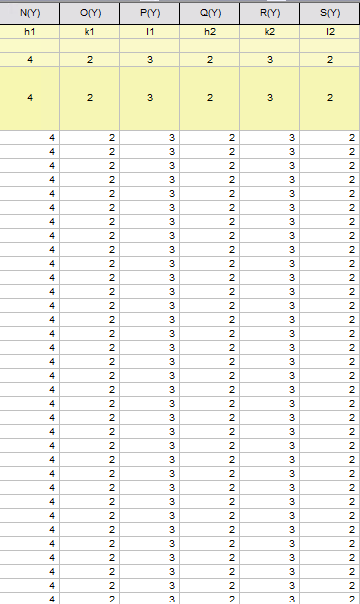
\includegraphics[width=\linewidth]{calc/c11.png}
    \caption{输入两组晶面指数}
    \label{fig:calc-rtheta-a}
  \end{subfigure}\hfill
  \begin{subfigure}[t]{0.70\linewidth}
    \centering
    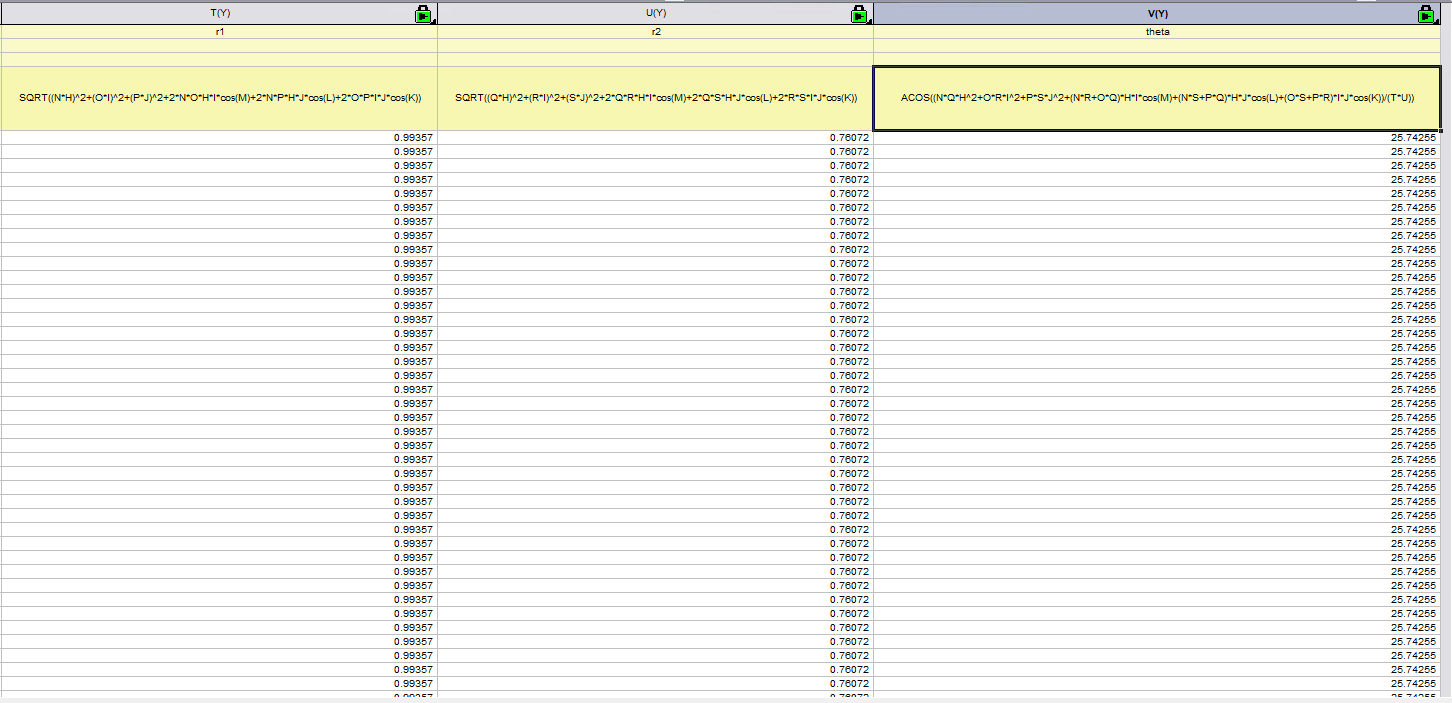
\includegraphics[width=\linewidth]{calc/c12.png}
    \caption{$r_1$、$r_2$ 与 $\theta$ 的计算结果}
    \label{fig:calc-rtheta-b}
  \end{subfigure}
  \caption{晶面组合的输入与 $r_1$、$r_2$、$\theta$ 的计算。T、U、V 三列分别对应式 \eqref{eq:rlength} 和式 \eqref{eq:angle}。}
  \label{fig:calc-rtheta}
\end{figure}

\subsection{单晶硅 PDF 卡片的构建}
\label{sec:cromer-mann}

PDF 卡片的核心信息是每一组衍射线的晶面指数 $hkl$、晶面间距 $d$、衍射角 $2\theta$ 和相对强度 $I/I_0$。在已建立的模板后面继续增加四列：$2\theta$、多重性 $N_{hkl}$、$|F_{hkl}|^2$ 和 $I/I_0$，即可把“晶体学计算器”扩展为“PDF 卡片生成器”；若需比较原子散射因子的影响，可再加一列 $I/I_0(f(s))$。

由 Bragg 方程 $2d\sin\theta=\lambda$ 得
\begin{equation}
2\theta=2\arcsin\left(\frac{\lambda}{2d_{hkl}}\right).
\label{eq:bragg}
\end{equation}
本作业取 Cu K$\alpha_1$ 波长 $\lambda=1.5406$~\AA。对粉末衍射，某一组 $\{hkl\}$ 的相对强度还正比于多重性 $N_{hkl}$ 和 Lorentz-偏振因子 $LP$：
\begin{equation}
I_{hkl}\propto N_{hkl}|F_{hkl}|^2LP,\qquad
LP=\frac{1+\cos^2 2\theta}{\sin^2\theta\cos\theta}.
\label{eq:intensity-powder}
\end{equation}
其中 $N_{hkl}$ 是同一 $d$ 值下等价晶面（包括交换和正负号）的数目。把表 \ref{tab:si-atoms} 的 8 个原子坐标代入式 \eqref{eq:structure-factor-simple}，即可得到 $|F_{hkl}|^2$；再用式 \eqref{eq:bragg} 和式 \eqref{eq:intensity-powder} 即可得到 $2\theta$ 和相对强度。表 \ref{tab:pdf-card} 列出了单晶硅的主要 PDF 卡片数据。

\begin{table}[H]
  \centering
  \caption{由计算模板得到的单晶硅 PDF 卡片数据（Cu K$\alpha_1$，$\lambda=1.5406$~\AA）}
  \label{tab:pdf-card}
  \small
  \setlength{\tabcolsep}{3pt}
  \renewcommand{\arraystretch}{1.05}
  \begin{tabular}{ccccccc}
    \toprule
    $hkl$ & $d$/\AA & $2\theta$/$^\circ$ & 多重性 & $|F|^2$ & $I/I_0$ ($f=14$) & $I/I_0$ ($f(s)$, $B=0.5$~\AA$^2$) \\
    \midrule
    111 & 3.1350 & 28.45 & 8  & 6272  & 100.0 & 100.0 \\
    220 & 1.9198 & 47.31 & 12 & 12544 & 98.0  & 64.3  \\
    311 & 1.6372 & 56.13 & 24 & 6272  & 66.4  & 37.3  \\
    400 & 1.3575 & 69.14 & 6  & 12544 & 21.0  & 9.6   \\
    331 & 1.2457 & 76.39 & 24 & 6272  & 34.8  & 14.1  \\
    422 & 1.1084 & 88.05 & 24 & 12544 & 57.1  & 19.4  \\
    511/333 & 1.0450 & 94.97 & 32 & 6272 & 36.2 & 11.1 \\
    440 & 0.9599 & 106.74 & 12 & 12544 & 27.9 & 7.2  \\
    531 & 0.9178 & 114.12 & 48 & 6272 & 60.3 & 14.0  \\
    620 & 0.8586 & 127.59 & 24 & 12544 & 76.4 & 15.1 \\
    533 & 0.8281 & 136.94 & 24 & 6272 & 47.8 & 8.6  \\
    444 & 0.7838 & 158.74 & 8  & 12544 & 69.2 & 10.6 \\
    \bottomrule
  \end{tabular}
\end{table}

表 \ref{tab:pdf-card} 中前一个强度列取 $f=14$，与第 3 章结构因子/消光系数计算的简化模型一致——$f$ 为原子散射因子，$14$ 即 Si 的原子序数，相当于只保留其前向散射值、忽略随角度的衰减（其含义与适用范围见第 \ref{sec:f14} 节）；后一个强度列把常数 $f$ 换成 Si 的 Cromer--Mann 原子散射因子 $f(s)$，并取温度因子 $B=0.5$~\AA$^2$，即
\begin{equation}
f(s)=\sum_{i=1}^{4}a_i e^{-b_i s^2}+c,\qquad s=\frac{\sin\theta}{\lambda}=\frac{1}{2d},
\label{eq:cromer-mann}
\end{equation}
其中 $a_1=6.2915$、$b_1=2.4386$，$a_2=3.0353$、$b_2=32.3337$，$a_3=1.9891$、$b_3=0.6785$，$a_4=1.5410$、$b_4=81.6937$，$c=1.1407$。$f(0)\approx14$，正好等于 Si 的原子序数，可作为系数是否抄对的检查。

表 \ref{tab:pdf-card} 与图 \ref{fig:pdf-card} 的数值由同一套公式算出，但作图方式不同：表格数据来自第 2.1--2.4 节的 Origin 模板（逐列输入晶格参数、$2\theta$、多重性和强度公式），而图 \ref{fig:pdf-card} 的棒图是用 \textbf{Python 3 + matplotlib} 编写的脚本自动生成的，没有在 Origin 中手工绘制。脚本的基本做法是：固定晶格常数、波长、常数 $f$ 和温度因子后，遍历 $0\le l\le k\le h\le 8$ 的 $hkl$，用式 \eqref{eq:structure-factor-simple} 求 $|F|^2$（为零即判为消光并剔除），用式 \eqref{eq:bragg} 求 $2\theta$、用式 \eqref{eq:intensity-powder} 求相对强度，按 $d$ 把退化组合（如 333 与 511）合并，归一化后用 \texttt{vlines} 画出两组棒图。

之所以用脚本而不是手工绘图，原因有三点：其一，PDF 卡片需要对上百个 $hkl$ 逐一枚举、按 $d$ 分组并统计多重性，手工录入既慢又容易漏项；其二，同一批数据要同时给出 $f=14$ 与 $f(s)$ 两套强度并排比较，脚本只需改一行常数即可重绘；其三，脚本可以同步打印表 \ref{tab:pdf-card} 的每一行，与 Origin 模板的结果逐行对照，起到交叉校验的作用（两者数值完全一致）。完整的构建思路、代码和运行方法见附录 C。若希望全部在 Origin 内完成，也可以把表 \ref{tab:pdf-card} 的 $2\theta$ 与强度两列直接画成柱状或棒状图，但枚举、分组和多重性统计仍建议由代码完成。

\begin{figure}[H]
  \centering
  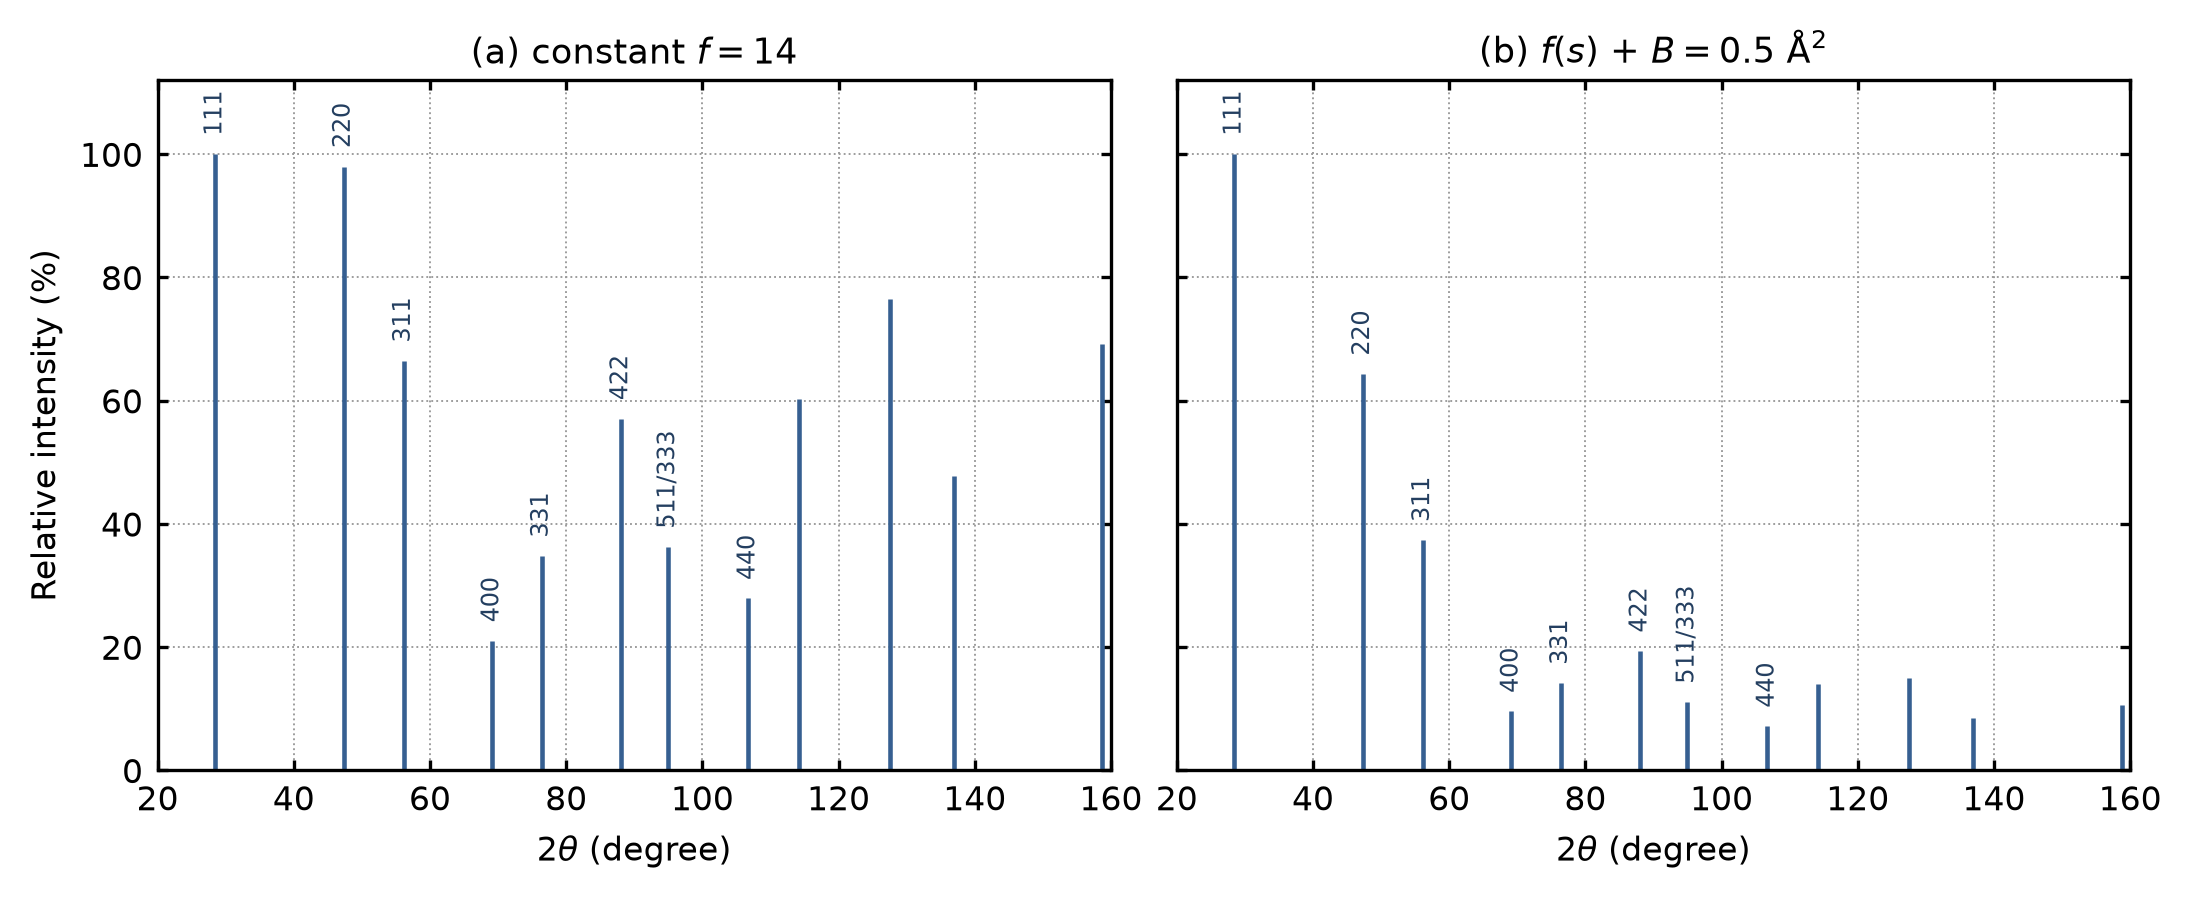
\includegraphics[width=\linewidth]{pdfcard.png}
  \caption{由计算模板得到的单晶硅 PDF 卡片棒图（Cu K$\alpha_1$）：(a) 常数原子散射因子 $f=14$；(b) 采用 Si 的 $f(s)$ 并取 $B=0.5$~\AA$^2$。两图的峰位完全相同，但高角反射的相对强度在后一模型中明显减弱。}
  \label{fig:pdf-card}
\end{figure}

从图 \ref{fig:pdf-card} 和表 \ref{tab:pdf-card} 可以看出：单晶硅最强的衍射线是 111，其次是 220、311、422 等；高角反射（如 531、620、444）在 $f=14$ 模型中仍然很强，而在 $f(s)$ 模型中显著减弱。这说明原子散射因子随 $\sin\theta/\lambda$ 增大而衰减，是 PDF 卡片强度计算中不可忽略的因素。标准 PDF 卡片还会进一步考虑温度因子、仪器几何、样品吸收、择优取向和结构精修等因素，因此表 \ref{tab:pdf-card} 给出的是运动学近似下的相对强度，而不是标准卡片的精确复制。把本文模板与标准卡片对照时，应重点比较 $d$ 和 $2\theta$ 的峰位，强度只作半定量参考。

\subsection{模板使用说明与常见错误}

把上述步骤固化为模板后，日常使用只需修改 A--F 列的晶格参数和 N--S 列的晶面指数，其余各列会自动更新。建议按以下顺序检查：

\begin{enumerate}[label=（\arabic*）,leftmargin=2.2em,itemsep=1pt]
  \item 确认角度单位为 Degree；
  \item 确认 A--F 列的晶格参数与目标物相一致，尤其是 $a,b,c$ 与 $\alpha,\beta,\gamma$ 的对应关系；
  \item 确认 H--M 列的公式引用的是正确的列（$a^*$ 用 $b,c,\alpha,V$，$b^*$ 用 $a,c,\beta,V$，$c^*$ 用 $a,b,\gamma,V$）；
  \item 确认 T--V 列的分母为 $r_1r_2$，且 $\theta$ 的分子中交叉项的系数为 $(h_1k_2+h_2k_1)$ 等，不要漏项；
  \item 用立方晶系的解析式 \eqref{eq:cubic-check} 抽查一两组数据；
  \item 制作 PDF 卡片时，确认 $2\theta$ 是由 $d$ 通过式 \eqref{eq:bragg} 得到的，而不是把 $\theta$ 直接当成 $2\theta$。
\end{enumerate}

最常见的错误有三类：一是角度单位误设为弧度，导致体积和夹角同时出错；二是公式中的列字母与列名不对应，复制公式后引用发生错位；三是结构因子求和时 \texttt{TOTAL} 的范围没有覆盖全部 8 个原子，或者把不同衍射点的原子行混在一起。第 3 章会在具体操作中再次强调这些检查点。
